\chapter{The Π-Ware library}
\label{chap:piware}

    Π-Ware is an \ac{EHDL} that allows for circuit description (modelling),
    simulation, reasoning (proving correctness or other properties), and synthesis to netlists.
    In this chapter we will describe in detail how the Π-Ware library is organized,
    what principles are behind some of the most important design decisions taken in its development,
    and how to use Π-Ware to model, simulate and reason about circuit behaviour.

    The reader is assumed to be familiar with the \emph{Agda} programming language,
    as this is the language in which Π-Ware is embedded.
    An introductory-level knowledge of dependent type theory in general is also appreciated.


    \section{Circuit Syntax}
    \label{sec:circuit-syntax}
        The most basic activity allowed by Π-Ware is the \emph{description} of circuits:
        as already mentioned briefly in the introduction, Π-Ware is \emph{deeply} embedded,
        which means there is a \emph{datatype} whose values are circuits.

        A deep embedding was chosen in order to allow for semantics other than execution (simulation).
        Particularly, the possibility of \emph{synthesizing} circuit models was a requirement
        kept in mind throughout the whole development.

        The circuit datatype (\AD{ℂ'}) is the most \emph{fundamental} of the whole library.
        It is defined as a dependent inductive family, indexed by two natural numbers,
        as shown in Listing~\ref{lst:Circuit-core}.

        \begin{listing}[h]
            \centering{\ExecuteMetaData[agda/latex/PiWare/Circuit/Core.tex]{Circuit-core}}
            \caption{The core circuit type (\AD{ℂ'}) of Π-Ware. \label{lst:Circuit-core}}
        \end{listing}

        A \emph{structural representation} of a circuit is achieved by the constructors of \AD{ℂ'}.
        This is in stark contrast with the the description style used in the Lava family, for example.
        In Lava, the constructors of the circuit datatype represent solely logic (or arithmetic) gates,
        and metalanguage (Haskell) constructs such as application, tupling and local naming are
        used to represent sequencing, parallel composition, loops and sharing.
        In Π-Ware, on the other hand, explicit constructors represent these combinations,
        avoiding the need to implement some form of \emph{observable sharing}~\cite{gill-typesafe-observable-sharing}.

        The indices of \AD{ℂ'} represent, respectively, the \emph{size} of the circuit's input and output.
        This can be thought of as the number of "wires" entering (resp. leaving) that circuit.
        Notice that the representation of inputs and outputs used in \AD{ℂ'} is untyped and unstructured.
        However, there is another – higher-level – circuit datatype (\AD{ℂ}),
        which adds a layer of typing \emph{on top} of \AD{ℂ'},
        and constitutes the actual intended \emph{interface} between the user (hardware designer) and Π-Ware.
        This abstraction layer will be discussed in more detail on Section~\ref{subsec:high-level-circuit}.

        To better understand the reasoning behind the design of the low-level \AD{ℂ'} datatype,
        its constructors can be considered to belong to one of three categories:

        \begin{description}
            \item[Fundamental:] These construct predefined or "atomic" circuits, with no sub-components.
                \begin{itemize}
                    \item \AI{Nil}: The \emph{empty circuit}. Performs no computation and has neither inputs nor outputs.
                        It is mainly useful as a "base case" when building large circuits with recursive definitions.
                    \item \AI{Gate}: Constructs a chosen circuit among those provided by a \emph{gate library}
                        passed as parameter to the \AM{Circuit} module.
                    \item \AI{Plug}: Constructs a "rewiring" circuit. Performs no computation,
                        but can be used to apply permutations, associativity and to duplicate or discard wires.
                \end{itemize}
            \item[Structural:] Represent ways in which smaller circuits can be interconnected to build a bigger one.
                \begin{itemize}
                    \item \AI{c₁ ⟫' c₂}: Sequential composition.
                        Given $c₁$ and $c₂$, connects the output of $c₁$ into the input of $c₂$.
                    \item \AI{c₁ |' c₂}: Parallel composition.
                        Splits the input into two parts, connected to $c₁$ and $c₂$,
                        and rejoins the outputs of $c₁$ and $c₂$ into a single output.
                    \item \AI{c₁ |+' c₂}: Tagged branching.
                        Based on the value of a \emph{tag} given in one of the input wires,
                        feed the remaining input wires into \emph{either} $c₁$ or $c₂$.
                \end{itemize}
            \item[Delay:]
                The \AI{DelayLoop} constructor belongs to a category of its own.
                Its purpose is to construct a state-holding circuit given a purely combinational circuit as argument.
        \end{description}

        These descriptions are just a rough summary of the \emph{synthesis semantics} of Π-Ware, that is,
        how each circuit constructor creates a netlist, given netlists as arguments.
        The precise \emph{definition} of the synthesis semantics is given in Section~\ref{sec:circuit-semantics}.
        The same section contains a detailed definition and explanation of a simulation semantics
        for Π-Ware circuits, both purely combinational and sequential ones.

        \subsection{Design discipline enforced by circuit constructors}
            The several constructors of \AD{ℂ'} "calculate" the port sizes of the circuits they construct,
            based on the sizes of the circuits given as arguments.
            These calculations implement \emph{structural well-formedness} rules for circuits.
            One example of such rule can be seen in the case of parallel composition:

            \begin{center}
                \begin{code}
                    \>[4]\AgdaInductiveConstructor{\_|'\_} \<[11]%
                    \>[11]\AgdaSymbol{:} \AgdaSymbol{∀} \AgdaSymbol{\{}\AgdaBound{i₁} \AgdaBound{o₁} \AgdaBound{i₂} \AgdaBound{o₂}\AgdaSymbol{\}} \<[30]%
                    \>[30]\AgdaSymbol{→} \AgdaDatatype{ℂ'} \AgdaBound{i₁} \AgdaBound{o₁} \AgdaSymbol{→} \AgdaDatatype{ℂ'} \AgdaBound{i₂} \AgdaBound{o₂} \AgdaSymbol{→} \AgdaDatatype{ℂ'} \AgdaSymbol{(}\AgdaBound{i₁} \AgdaPrimitive{+} \AgdaBound{i₂}\AgdaSymbol{)} \AgdaSymbol{(}\AgdaBound{o₁} \AgdaPrimitive{+} \AgdaBound{o₂}\AgdaSymbol{)}\<%
                \end{code}
            \end{center}

            In this case, the input (resp. output) size of the composed circuit equals the \emph{sum}
            of the input (resp. output) sizes of the constituent sub-circuits.
            Other such rules are also imposed by \AI{\_⟫'\_}, \AI{\_|+'\_} and \AI{Plug}.
            Together, all of them ensure:

            \begin{description}
                \item[No floating wires] Circuit sizes need to match in order for the usage of a constructor
                    to be type-correct. In particular, no circuit \emph{input} wires are ever left \emph{disconnected}.
                    Figure~\ref{fig:sequencing-floating} illustrates an example of a situation banned by the sizing rule present
                    in the type of \AI{\_⟫'\_}.

                    \begin{figure}[h]
                        \centering{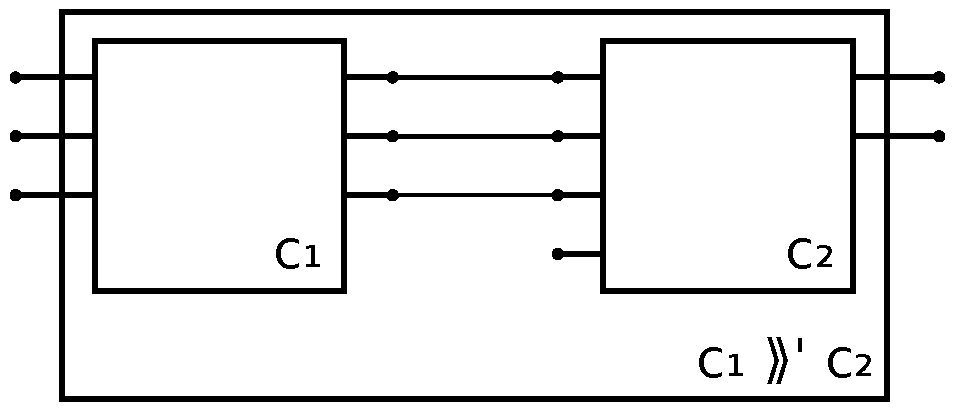
\includegraphics[width=0.6\textwidth]{imgs/sequencing-floating.pdf}}
                        \caption{Example of circuit banned by the type of \AI{\_⟫'\_}.\label{fig:sequencing-floating}}
                    \end{figure}

                \item [No short-circuits] The \AI{Plug} constructor, the only one which can be used for
                    "rewiring" purposes, has a type which forbids connecting multiple sources to the same load.
                    Its argument is a \emph{function from outputs to inputs}.
                    In this way, definitions connecting multiple inputs to the same output are banned,
                    as they are \emph{not} functions from outputs to inputs.
                    Also, when a plug is used between two sub-circuits $c₁$ and $c₂$,
                    a definition in which an \emph{input} of $c₂$ would be left \emph{disconnected} is disallowed by Agda,
                    as such a definition would not be \emph{total}.
                    The diagram on Figure~\ref{fig:plug-seq-disconnected-input} represents such a banned situation:

                    \begin{figure}[h]
                        \centering{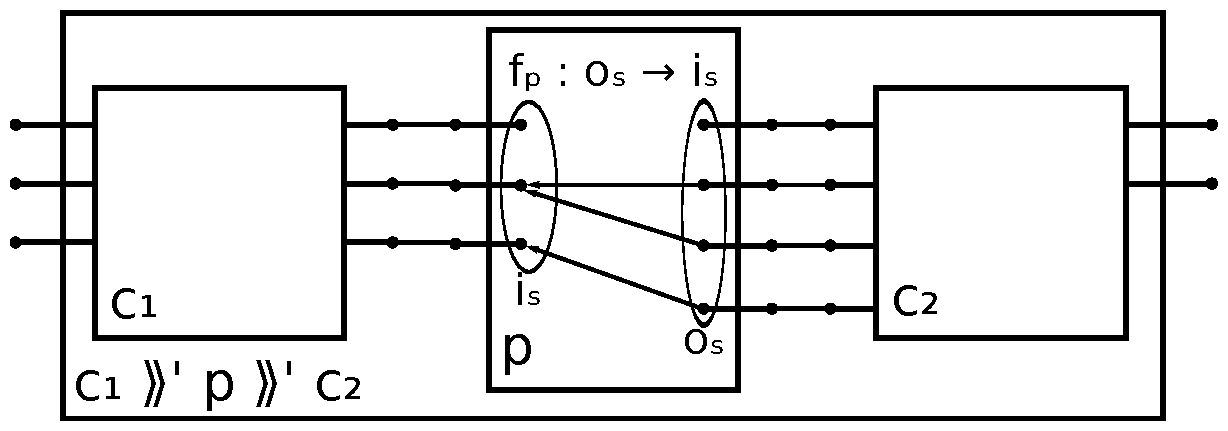
\includegraphics[width=0.8\textwidth]{imgs/plug-seq-disconnected-input.pdf}}
                        \caption{This circuit cannot be constructed because $f_{p}$ is not \emph{total}.\label{fig:plug-seq-disconnected-input}}
                    \end{figure}
            \end{description}

            \subsubsection{Purely combinational vs. possibly sequential}
            Another piece of information "carried" together with circuits is whether it is
            \emph{purely combinational}, i.e., has no internal state, no notion of \emph{history},
            and the value of its current outputs depend only on the value of its current inputs.

            This information is represented by a metalanguage truth value,
            an Agda \AF{Set} which can be either \AF{⊤} (the \AF{Set} with one value – "top") or
            \AF{⊥} (the \AF{Set} with no values – "bottom").

            The predicate \AF{comb'} over low-level (\AF{ℂ'}) circuits defines whether a circuit purely combinational.
            The code for \AF{comb'} is shown on Listing~\ref{lst:comb-core}.

            \begin{listing}[h]
                \centering{\ExecuteMetaData[agda/latex/PiWare/Circuit/Core.tex]{comb-core}}
                \caption{Predicate telling whether a low-level circuit is purely combinational.\label{lst:comb-core}}
            \end{listing}

            Notice that the fundamental constructors \AI{Nil}, \AI{Gate} and \AI{Plug} \emph{always}
            build purely combinational circuits, while \AI{DelayLoop} always produces circuits with internal state.
            The structural constructors (\AI{\_⟫'\_}, \AI{\_|'\_} and \AI{\_|+'\_})
            yield a purely combinational circuit if and only if \emph{both} of its argument are themselves purely combinational.
            This is expressed by using the product type constructor \AF{\_×\_}, which in the \AF{Set}
            level corresponds to a logical conjunction.

            This categorization of circuits as stateful or stateless has one main goal:
            To avoid the evaluation of \emph{combinational loops}.
            Their presence in a circuit is almost always a design mistake, and by combining
            the \AI{DelayLoop} constructor with the \AF{comb'} predicate we guarantee that:

            \begin{itemize}
                \item The only way to create a loop in a circuit (\AI{DelayLoop}) also introduces a delay.
                \item Combinational simulation (ignoring past inputs) only happens when safe.
            \end{itemize}


    \section{Abstraction Mechanisms}
    \label{sec:circuit-abstraction}
        Several of the definitions (modules, datatypes, functions) of Π-Ware
        are parameterized in order to improve code reuse.
        The library allows for a choice of the type of data carried in individual wires,
        the types that serve as inputs and ouputs to circuits,
        and the set of fundamental gates from which circuits are built.

        In this section we present how this flexibility is achieved,
        and which requirements are imposed upon the parameters in each case of parameterization.
        Also, the motivation behind the chosen requirements is presented,
        based on the general goals of Π-Ware as well as the wish to impose as few constraints as possible.


        \subsection{Atoms}
        \label{subsec:atoms}
            In \acp{EDSL} of the current Lava family~\cite{observable-sharing-circuits},
            only values of type \mintinline{haskell}{Bool} and \mintinline{haskell}{Int}
            can be carried by the "wires", and circuits can only operate on inputs and outputs
            which are tuples or lists of these basic types.

            There is a little more flexibility in ForSyDe~\cite{forsyde1999},
            where the \mintinline{haskell}{ProcType} type class determines what types can be used
            as input and output types of \emph{process functions} (combinational circuits).
            ForSyDe has predefined instances of \mintinline{haskell}{ProcType} for fixed-width numeric types
            (\mintinline{haskell}{Int8}, \mintinline{haskell}{Int16}, etc.) and \mintinline{haskell}{Bool},
            while relying on \emph{Template Haskell} to generate instances for user-defined \emph{enumeration types}
            at compile time.

            Π-Ware's approach is similar to ForSyDe's, in that it shares the same goal
            (to "carry" in the wires any type that belongs to a type class).
            However, Π-Ware does not use any metaprogramming, and uses dependent types
            to ensure that the provided instances satisfy desired properties.
            The type class \AD{Atomic} (shown in Listing~\ref{lst:atomic})
            expresses in Π-Ware what are the requirements for a type to be carried in the wires of a circuit.

            \begin{listing}[h]
                \centering{\ExecuteMetaData[agda/latex/PiWare/Atom.tex]{Atomic}}
                \caption{The \AD{Atomic} type class.\label{lst:atomic}}
            \end{listing}

            The fields \AL{Atom} and \AL{|Atom|-1} determine, respectively,
            the Agda \AD{Set} to be used as basis and \emph{how many elements} of this \AD{Set}
            are to be used as atoms (the number of atoms is actually \AF{|Atom|} \AY{=} \AI{suc} \AL{|Atom|-1}).

            Then there are the fields \AL{n→atom} and \AL{atom→n}, which define a \emph{bijection}
            between the \AL{Atom} type and \AD{Fin} \AF{|Atom|} (naturals from \AI{zero} to \AF{|Atom|}).
            Finally, the two last fields in \AF{Atomic} are proofs
            that \AL{n→atom} and \AL{atom→n} are inverses of each other,
            therefore proving that they are also bijections.

            \subsubsection{Instance for \texttt{Bool}}
            Included with Π-Ware there is already a predefined instance of \AD{Atomic} for \AD{Bool}
            (the boolean type in Agda's standard library).
            Knowing the meaning of each field, the definitions comprising the instance
            are mostly easy to understand.
            First, we start by defining the cardinality of the set of values we are interest in
            (\AD{B} is used as synonym for \AD{Bool}):

            \begin{center}
                \ExecuteMetaData[agda/latex/PiWare/Atom/Bool.tex]{cardinality}
            \end{center}

            Now, before defining the bijections that enumerate the set of atoms,
            we give more convenient \emph{names} to the elements of \AD{Fin} \AF{|B|} used in the enumeration
            by using an Agda feature known as \emph{pattern synonyms}:

            \begin{center}
                \ExecuteMetaData[agda/latex/PiWare/Atom/Bool.tex]{pattern-synonyms}
            \end{center}

            The usage of the \AI{Absurd\#} pattern becomes clearer when we take a look at
            the definitions of the bijections themselves:

            \begin{center}
                \ExecuteMetaData[agda/latex/PiWare/Atom/Bool.tex]{nToBool}
            \end{center}

            In the case of the \AI{Absurd\#} pattern, there is no need to provide a right-hand side
            to the equation, as the Agda typechecker can verify that
            there is no \AB{x} such that \AI{Fs} \AY{(}\AI{Fs} \AB{x}\AY{)} belongs to \AD{Fin} \AN{2}.

            Finally, there are the proofs stating that \AF{n→B} has a two-sided inverse (namely, \AF{B→n}),
            and, therefore, it is a bijection. The proofs use simple case analysis (and reflexivity).

            \begin{center}
                \ExecuteMetaData[agda/latex/PiWare/Atom/Bool.tex]{inv-Bool}
            \end{center}

            \subsubsection{Other possibly interesting instances}
            Even though currently \AD{Bool} (from the Agda standard library) is the only type for which
            there is already a predefined instance of \AD{Atomic}, other types could be interestingly used as atoms.
            For example:

            \begin{description}
                \item[Three-valued logic types]
                    Representing the values \texttt{TRUE}, \texttt{FALSE} and \texttt{UNKNOWN}
                \item[IEEE1164 nine-valued logic]
                    Standardized logic used widely in industry as a VHDL/Verilog type.
                    Besides the usual \texttt{FALSE} and \texttt{TRUE} logical values
                    (represented respectively by '0' and '1'),
                    it accomodates also the following others:
                    \begin{itemize}
                        \item \texttt{'Z'}: \emph{High impedance}, means output is not being driven.
                        \item \texttt{'X'}: \emph{Strong drive, unknown logic value}.
                        \item \texttt{'W'}: \emph{Weak drive, unknown logic value}.
                        \item \texttt{'L'}: \emph{Weak drive, logic zero}.
                        \item \texttt{'H'}: \emph{Weak drive, logic one}.
                        \item \texttt{'U'}: \emph{Uninitialized}. Used as default initial value in simulation.
                        \item \texttt{'-'}: \emph{Don't care}.
                    \end{itemize}
            \end{description}


        \subsection{Gate library}
        \label{subsec:gate-library}
            Besides being parameterized by the type of \AD{Atom}s that can be carried in their wires,
            Π-Ware low-level circuit descriptions (\AD{ℂ'}) are also parameterized by
            a \emph{library of fundamental gates} upon which circuits are built.

            There are several interesting possible gate libraries which could be used to describe circuits,
            among which:

            \acrodef{DSP}{Digital Signal Processing}
            \begin{itemize}
                \item \emph{Functionally complete} sets of boolean functions such as
                    $\{ \text{\texttt{NAND}} \}$, $\{ \text{\texttt{NOR}} \}$ or
                    $\{ \text{\texttt{NOT}}, \text{\texttt{AND}}, \text{\texttt{OR}} \}$
                    (predefined in the Π-Ware library).
                \item Arithmetic primitives over boolean vectors, such as $\{ \text{\texttt{\_+\_}}, \text{\texttt{\_*\_}} \}$.
                \item A logic-arithmetic library together with some purpose-specific primitives,
                    for example cryptographic and \ac{DSP} functions.
            \end{itemize}

            A gate library is defined as an element of the \AD{Gates} record type, shown in Listing~\ref{lst:gates}.

            \begin{listing}[h]
                \centering{\ExecuteMetaData[agda/latex/PiWare/Synthesizable.tex]{Word}}
                \newline
                \centering{\ExecuteMetaData[agda/latex/PiWare/Gates.tex]{Gates}}
                \caption{Definition of a gate library: the \AD{Gates} record.\label{lst:gates}}
            \end{listing}

            The first field of the \AD{Gates} record (\AL{|Gates|-1}) determines \emph{how many}
            gates the library has, and consequently also the \emph{the type used as gate index}
            (or \emph{gate identifier}), which is \AF{Gates\#} \AY{=} \AF{Fin} \AF{|Gates|}.

            For each gate identifier, the functions \AL{ins} and \AL{outs} determine, respectively,
            the size of the input and output of that gate; therefore together they determine the gate's \emph{interface}.

            Finally, the \AL{spec} field determines the \emph{functional specification} of a given gate identifier.
            Notice how the whole \AM{Gates} module is parameterized by an instance of \AD{Atomic}.
            In this way, the \AL{spec} function yields, given a gate identifier, a function over \emph{words}
            (\AD{Atom} vectors) of the correct length.
            This functional specification of each fundamental gate is used for the \emph{simulation semantics}.

            \subsubsection{Assumed correctness}
            Later, in Section~\ref{sec:proving-circuit-properties}, we will give a precise definition
            for what is considered the \emph{functional correctness} of a circuit; its \emph{compliance}
            to a certain functional specification.

            Usually, the proof of functional correctness for a circuit is built using, in some way,
            the correctness proofs of its subcomponents.
            However, fundamental gates have no subcomponents, so their correctness is assumed.
            By definition, the simulation semantics of a fundamental gate is equal to the \AL{spec}
            function given for it in the gate library definition.

            \subsubsection{Relation to synthesis}
            \label{subsubsec:relation-to-synthesis}
            Even though fundamental gates have no subcomponents \emph{at the Π-Ware level},
            they are not in any way directly synthesizable to \ac{VHDL}.
            To convert a Π-Ware circuit to \ac{VHDL}, each fundamental gate in the library being used
            needs to have a corresponding excerpt of \ac{VHDL} code representing it.

            This feature is not integrated in the current version of Π-Ware, but assuming the existence
            of a hierarchy of datatypes representing \ac{VHDL} code, and specifically the existence
            of a type \AD{VHDLEntity}, we could have an extra field in the \AD{Gates} record, as such:

            \begin{center}
               \AL{netlist} \AY{:} \AY{(}\AB{g} \AY{:} \AD{Fin} \AY{(}\AI{suc} \AL{|Gates|-1}\AY{)}\AY{)} \AY{→} \AD{VHDLEntity} \AY{(}\AL{ins} \AB{g}\AY{)} \AY{(}\AL{out} \AB{g}\AY{)}
            \end{center}

            The \AD{VHDLEntity} is also parameterized by the input and output sizes of the circuit,
            tying the Π-Ware fundamental gate interface with the \ac{VHDL} abstract syntax.

            \subsubsection{Instance for \texttt{BoolTrio}}
            One specific instance of gate library is already "shipped" with Π-Ware:
            the usual set of boolean gates
            $\{ \text{\texttt{NOT}}, \text{\texttt{AND}}, \text{\texttt{OR}} \}$, together with
            the constants $\{ \text{\texttt{FALSE}}, \text{\texttt{TRUE}} \}$.
            The first definitions establish that this library contains five gates:

            \begin{center}
                \ExecuteMetaData[agda/latex/PiWare/Gates/BoolTrio.tex]{cardinality}
            \end{center}

            Then, as already done in the instance of \AD{Atomic}, we define some \emph{pattern synonyms}
            to make the gate identifiers more readable:

            \begin{center}
                \ExecuteMetaData[agda/latex/PiWare/Gates/BoolTrio.tex]{pattern-synonyms}
            \end{center}

            The next step is to define the \emph{interface} of each gate in the library.
            All gates have exactly one output, while the number of inputs vary from 0 to 2.

            \begin{center}
                \ExecuteMetaData[agda/latex/PiWare/Gates/BoolTrio.tex]{ins-outs}
            \end{center}

            Finally, the last piece of information needed to define the gate library is
            the functional specification of each gate.

            \begin{center}
                \ExecuteMetaData[agda/latex/PiWare/Gates/BoolTrio.tex]{spec}
            \end{center}

            Notice that the gates use \AD{Bool} from Agda's standard library as their \AD{Atom} type.
            Also the logic operators from the standard library (\AM{Data.Bool}) are used in the specification.
            With all the necessary pieces of the puzzle in hand, the definition of the \AD{BoolTrio}
            gate library is as follows:

            \begin{center}
                \ExecuteMetaData[agda/latex/PiWare/Gates/BoolTrio.tex]{BoolTrio}
            \end{center}


        \subsection{High-level circuit datatype}
        \label{subsec:high-level-circuit}
            When presenting the low-level circuit datatype (\AD{ℂ'}) on Section~\ref{sec:circuit-syntax},
            it was mentioned that the representation using \AD{ℂ'} is untyped and unstructured, i.e.,
            all circuit inputs and outputs at that level are just sequences of \AD{Atom}s (for example, bits).

            However, the user of Π-Ware is not supposed to actually model circuits using the \AD{ℂ'} datatype.
            There is a layer of abstraction sitting on top of \AD{ℂ'},
            and circuits at this higher level have inputs and outputs with Agda types.
            This layer is coded as the \AD{ℂ} datatype, shown in Listing~\ref{lst:Circuit}.

            \begin{listing}[h]
                \centering{\ExecuteMetaData[agda/latex/PiWare/Circuit.tex]{Circuit}}
                \caption{High-level circuit datatype (\AD{ℂ}).\label{lst:Circuit}}
            \end{listing}

            First of all, notice the \emph{lack of a prime symbol in the name of the datatype}.
            This is a general naming convention:
            whenever there are two versions of a definition, one at a low level of abstraction and one higher,
            the low-level gets the same name of the high-level one, with a prime symbol as suffix.

            In contrast to the low-level (\AD{ℂ'}) circuit type, \AD{ℂ} is parameterized by two Agda \AD{Set}s,
            and has only one constructor – \AI{Mkℂ} – which "packs" the low-level circuit description
            with the information on how to convert between the input/output Agda types
            (resp. \AB{α} and \AB{β}) and the appropriately-sized \emph{words} used in the low level.
            This conversion information is coded in the \AD{⇓𝕎⇑} type class (pronounced \texttt{Synthesizable}),
            which is covered in more detail on Section~\ref{subsec:synthesizable}.

            Furthermore, the \AM{PiWare.Circuit} module defines also \emph{smart constructors} for \AD{ℂ},
            corresponding to each of the constructors at the low level.
            One example is parallel composition:

            \begin{center}
                \ExecuteMetaData[agda/latex/PiWare/Circuit.tex]{par}
            \end{center}

            Using a \emph{gate library} together with these smart constructors, one can model
            hardware circuits operating over Agda types.
            One very simple example is a \texttt{XOR} circuit (shown in Listing~\ref{lst:xor-sample}),
            built using the \texttt{BoolTrio} gate library mentioned before.
            The block diagram in Figure~\ref{fig:xor-sample} illustrates the architecture of such circuit.

            \begin{figure}[h]
                \centering{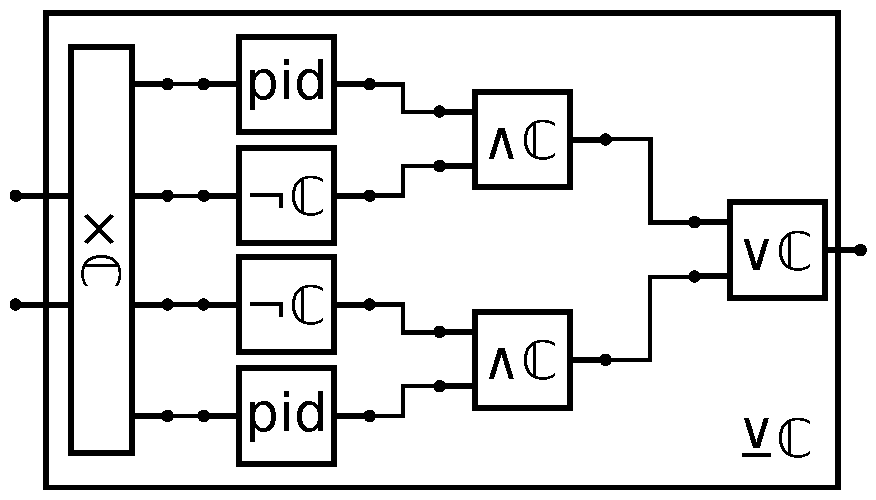
\includegraphics[width=0.50\textwidth]{imgs/xor-sample.pdf}}
                \caption{Architecture of a sample \texttt{XOR} gate.\label{fig:xor-sample}}
            \end{figure}

            \begin{listing}[h]
                \centering{\ExecuteMetaData[agda/latex/PiWare/Samples/BoolTrioComb.tex]{fundamentals}}
                \newline
                \centering{\ExecuteMetaData[agda/latex/PiWare/Samples/BoolTrioComb.tex]{xor}}
                \caption{Example of a \texttt{XOR} gate built with the \texttt{BoolTrio} library.\label{lst:xor-sample}}
            \end{listing}

            Again in this example, as customary, we renamed \AD{Bool} to \AD{B},
            and \AF{pid} is the \emph{identity plug}.
            The identity plug can be substituted in the netlist by a \emph{bus} (with the adequate size),
            and is defined (together with other useful plugs) in the \AM{PiWare.Plugs} module.


        \subsection{The \texttt{Synthesizable} type class}
        \label{subsec:synthesizable}
            The "connection" between the low-level (\AD{ℂ'}) and high-level (\AD{ℂ}) circuit types
            is done by the \AD{⇓𝕎⇑} type class (pronounced \texttt{Synthesizable}).
            Instances of the \AD{⇓𝕎⇑} class define a mapping between a given Agda type
            and an appropriately-sized \emph{word} type.
            Word types (\AD{𝕎} \AB{n}, for some \AB{n}) are \emph{synthesizable} to \ac{VHDL} vectors,
            thus the name of the class.
            Listing~\ref{lst:Synth} shows the definition of \AD{⇓𝕎⇑}:

            \begin{listing}[h]
                \centering{\ExecuteMetaData[agda/latex/PiWare/Synthesizable.tex]{Word}}
                \newline
                \centering{\ExecuteMetaData[agda/latex/PiWare/Synthesizable.tex]{Synth}}
                \caption{The \AD{⇓𝕎⇑} (Synthesizable) type class.\label{lst:Synth}}
            \end{listing}

            The type class has two parameters: the type which it encodes (\AB{α}),
            and the size of the \emph{word type} to which \AB{α} corresponds (\AB{i}).
            Notice that the size parameter is passed \emph{implicitly}, because in some occasions
            Agda might be able to automatically infer (by unification) this value.

            One can imagine that all \emph{finite types} (types with finitely many elements)
            can be made synthesizable under the definition of \AD{⇓𝕎⇑}, given a certain encoding scheme.
            We do not give a proof of this statement, but one way of doing it would be to translate
            Agda datatype definitions into a sum-of-products view and then use a standardized
            encoding scheme (for example, some form of \emph{Church encoding}).

            Π-Ware does \emph{not} provide facilities for mapping arbitrary Agda datatypes into
            a sum-of-products view (we believe this is the domain of a \emph{generic programming} library,
            not of a hardware \ac{EDSL}).
            However, Π-Ware \emph{does} provide predefined instances of \AD{⇓𝕎⇑} for units (\AD{⊤}),
            booleans (\AD{Bool}), products (\AD{\_×\_}), vectors (\AD{Vec}) and sums (\AD{\_⊎\_}),
            in order to facilitate working with complex types when modelling hardware.

            One interesting instance to look at is the one for Agda's standard library vectors (\AD{Vec}),
            shown in Listing~\ref{lst:Synth-Vec}.

            \begin{listing}[h]
                \centering{\ExecuteMetaData[agda/latex/PiWare/Synthesizable.tex]{Synth-Vec}}
                \caption{Predefined instance of \AD{⇓𝕎⇑} for fixed-length vectors.\label{lst:Synth-Vec}}
            \end{listing}

            In the \AF{down} definition,
            the \emph{bind} (\AF{>>=}) operator is defined as \AF{concat} \AO{∘} \AF{map}, i.e.,
            first each element of the vector is serialized (using the passed instance for \AB{α}),
            then all the words (each with size \AB{i}) are concatenated, giving a total size of
            \AY{(}\AB{n} \AF{*} \AB{i}\AY{)}.

            To convert a serialized \AD{Vec} back \AF{up}, first the given word is \AF{group}ed
            into \AB{n} smaller words (each of size \AB{i}), which is possible because the size of
            the passed word is \AY{(}\AB{n} \AF{*} \AB{i}\AY{)}.
            Then, ignoring the proof object returned by \AF{group} (which is in the second position
            of a pair, therefore we take \AL{proj₁}), we map the \AF{up} instance of \AB{α} over
            each of the smaller words, obtaining in this way an element of type
            \AD{Vec} \AB{α} \AB{n}.

            \subsubsection{Proof of bijection}
            It is very desirable that the pair of fields "down" (\AL{⇓}) and "up" (\AL{⇓}),
            for any instance of \AD{⇓𝕎⇑}, are inverses of each other, that is:

            \begin{center}
                \AY{∀} \AY{(}\AB{x} \AY{:} \AB{α}\AY{)} \AY{→} \AL{⇑} \AY{(}\AL{⇓} \AB{x}\AY{)} \AF{≡} \AB{x}
                \\
                \AY{∀} \AY{(}\AB{w} \AY{:} \AD{𝕎} \AB{i}\AY{)} \AY{→} \AL{⇓} \AY{(}\AL{⇑} \AB{w}\AY{)} \AF{≡} \AB{w}
            \end{center}

            We indeed tried to embed these proofs also as methods of the \AD{⇓𝕎⇑} class.
            However, when trying to write the proofs for the included instances,
            we faced some difficulties (especially in the sum case) and left this endeavour for future work
            (discussed in more detail in Section~\ref{subsec:current-limitations}.

            \subsubsection{\texttt{Synthesizable} instance for sums}
            The instance of \AD{⇓𝕎⇑} for sums (disjoint unions) is the most complex among all predefined
            instances included with Π-Ware.
            This complexity comes mostly from the need to \emph{distinguish} which set is concerned
            when converting a word "up" (\AL{⇑}).
            Assuming that we want \AL{⇓} and \AL{⇑} to form a bijection (no information may be lost),
            let's first calculate how many atoms are necessary to represent a sum.

            With a given encoding for set \AB{α} (\AB{sα} \AY{:} \AD{⇓𝕎⇑} \AB{α} \AY{\{}\AB{i}\AY{\}})
            and one for β (\AB{sβ} \AY{:} \AD{⇓𝕎⇑} \AB{β} \AY{\{}\AB{j}\AY{\}}),
            it is clear that at least \AB{i} \AF{⊔} \AB{j} atoms are necessary to encode \AB{α} \AD{⊎} \AB{β};
            the size of a sum is at least the maximum among the sizes of its summands.
            Furthermore, it is necessary to somehow encode the choice (whether the sum was built from
            the left (\AL{inj₁}) or the right (\AL{inj₂}). This requires at least one more atom,
            bringing the size to \AI{suc} \AY{(}\AB{i} \AF{⊔} \AB{j}\AY{)}.

            The predefined instance for sums included with Π-Ware is shown on Listing~\ref{lst:Synth-Sum}.

            \begin{listing}[h]
                \centering{\ExecuteMetaData[agda/latex/PiWare/Synthesizable.tex]{Synth-Sum}}
                \caption{Predefined instance of \AD{⇓𝕎⇑} for sums.\label{lst:Synth-Sum}}
            \end{listing}

            Besides the encodings of the summands (named \AB{sα} and \AB{sβ},
            given as \emph{instance arguments}), this instance is also passed some extra parameters:
            three \emph{atom indices} (\AB{n}, \AB{m} and \AB{p}) and a proof that \AB{n} and \AB{m} are different.
            The atom index \AB{n} indicates the \AD{Atom} to be used in case the sum is built from the left (\AL{inj₁}).
            and \AB{m} for the case when it is built from the right (\AL{inj₂}).
            They need to be different in order for the choice information not to be lost when synthesizing a sum.
            At last, the \AB{p} parameter identifies the atom used for padding.

            In the \AF{down} function, the \AF{[\_,\_]} sum \emph{destructor} is used,
            and is passed two functions: one to operate at the left case and one at the right.
            They prepend to the output word an atom identified by either \AB{n} or \AB{m} and pad
            either \AB{a} or \AB{b} to fit \AB{i} \AF{⊔} \AB{j}.

            In the \AF{up} conversion, first the \emph{tag} is used to transform the input word into
            a sum of words (\AD{𝕎} \AB{i} \AD{⊎} \AD{𝕎} \AB{j}),
            then the \AF{map⊎} function is used to apply either the \AL{⇑} instance for \AB{α} or for \AB{β},
            giving the desired result type of \AB{α} \AD{⊎} \AB{β}.

            \subsubsection{Recursive instance search}
            To model synthesizable datatypes, we used the Agda way of implementing Haskell's type classes,
            namely, to code a type class as a record type, in which each field corresponds to a method.
            In this analogy, instances are just elements of the record type, and class constraints are
            coded in Agda by passing \emph{instance arguments}~\cite{typeclasses-agda} to the constrained function.
            Arguments passed in this way will be searched among the identifiers available in scope,
            in a type-directed fashion, similar to how the mechanism of instance search works in Haskell.

            However, there was (until recently) a big drawback to Agda's instance search implementation:
            it was not recursive.
            There were some arguments for this decision in the seminal paper,
            most notably that having fully recursive instance resolution would
            "expose an additional computational model" and that the instance search mechanism
            would need to "perform a reasonably powerful automated proof search".

            During the last years, since the publication of the paper on instance arguments~\cite{typeclasses-agda},
            demand has grown for recursive instance search in Agda, and in a recent contribution to the Agda codebase
            by Guillaume Brunerie~\footnote{\url{https://github.com/agda/agda/commit/7ca60fd60aec1b73d9f14aaa6e1aeef184bcca79}},
            costs and benefits were again weighted, and a reasonably efficient implementation was released
            in Agda version 2.4.0.2 (current version at the time of writing this report).

            The impact of this change for Π-Ware is immense.
            Recursive instance resolution removes the need for a great deal of boilerplate code.
            For example, before the advent of recursive resolution, modelling the \texttt{XOR} circuit
            on Listing~\ref{lst:xor-sample} required the user to manually construct instances of \AD{⇓𝕎⇑}
            for more than 5 types
            ( \AD{𝔹} \AD{×} \AD{𝔹}
            , \AY{(}\AD{𝔹} \AD{×} \AD{𝔹}\AY{)} \AD{×} \AD{𝔹}
            , \AD{𝔹} \AD{×} \AY{(}\AD{𝔹} \AD{×} \AD{𝔹}\AY{)}
            , \AY{(}\AD{𝔹} \AD{×} \AY{(}\AD{𝔹} \AD{×} \AD{𝔹}\AY{)}\AY{)} \AD{×} \AY{(}\AD{𝔹} \AD{×} \AD{𝔹}\AY{)}
            , etc.).
            Now all of this work is done by Agda itself.
            On the other hand, the typechecking time grew a little,
            and this could be a problem when modelling big circuits, as discussed in Section~\ref{subsec:current-limitations}.


    \section{Circuit Semantics}
    \label{sec:circuit-semantics}
        In this chapter we will expose and discuss the \emph{semantics} of circuits described using Π-Ware.
        Namely, Π-Ware circuits can be interpreted in two ways:
        they can be \emph{simulated} (fed with certain inputs and calculate the correspoding outputs)
        or \emph{synthesized} (converted to a \emph{netlist}).

        When presenting the simulation semantics, we will separately discuss the simulation of
        purely combinational circuits and of sequential ones,
        also recapitulating the need to distinguish between the two.

        \subsection{Synthesis semantics}
        \label{subsec:synthesis-semantics}
            The synthesis semantics establishes how Π-Ware circuits can be converted to netlists.
            Each element of the low-level circuit datatype (\AD{ℂ'}) has a corresponding netlist
            according to the semantics,
            and to each circuit constructor corresponds a netlist transformation.

            Figure~\ref{fig:semantics-syn-fundamental} shows the semantic rules for the
            fundamental constructors of \AD{ℂ'}, as well as for \AI{DelayLoop}.
            To the left of each diagram there is a typing rule for that case,
            with the constructor's arguments (and their types) above the bar and the result type below it.

            \begin{figure}[h]
                \centering{\includegraphics[width=0.93\textwidth]{imgs/semantics-syn-fundamental.pdf}}
                \caption{Synthesis semantics of the fundamental circuit constructors.\label{fig:semantics-syn-fundamental}}
            \end{figure}

            In the diagrams, all ellipses denote elements of type \AD{ℂ'}, i.e., low-level circuits.
            Assuming the existence of a hierarchy of datatypes for representing \ac{VHDL} code
            (as already mentioned in Section~\ref{subsubsec:relation-to-synthesis}),
            each of these ellipses correspond to a \ac{VHDL} \emph{entity} (an element of \AD{VHDLEntity}).

            The line segments connecting the ellipses are signals (\AD{VHDLSignal}) – with their size
            denoted by the variable above the perpendicular "dash" in the segment.
            Each of the little dots on the extremity of a line segment correspond to a \emph{port declaration}
            (\AD{VHDLPortDecl}). The arrows on the line segments indicate the direction of the flow of information.

            \acrodef{FPGA}{Field-Programmable Gate Array}
            It is important that these diagrams \emph{do not prescribe any placement} for the circuit components.
            They denote only \emph{netlists}, i.e., directed graphs in which the nodes are elements of \AD{ℂ'}
            and the edges are the signals connecting them (labeled by signal \emph{size}).
            The actual \emph{placement} of this netlist into physical slots (of an \ac{FPGA} or \ac{ASIC}),
            with the accompanying \emph{routing} of wires, is a further step in the implementation chain,
            \emph{not performed by Π-Ware}.

            The semantics of structural circuit constructors (sequential, parallel, sum) is
            shown in Figure~\ref{fig:semantics-syn-structural}.

            \begin{figure}[h]
                \centering{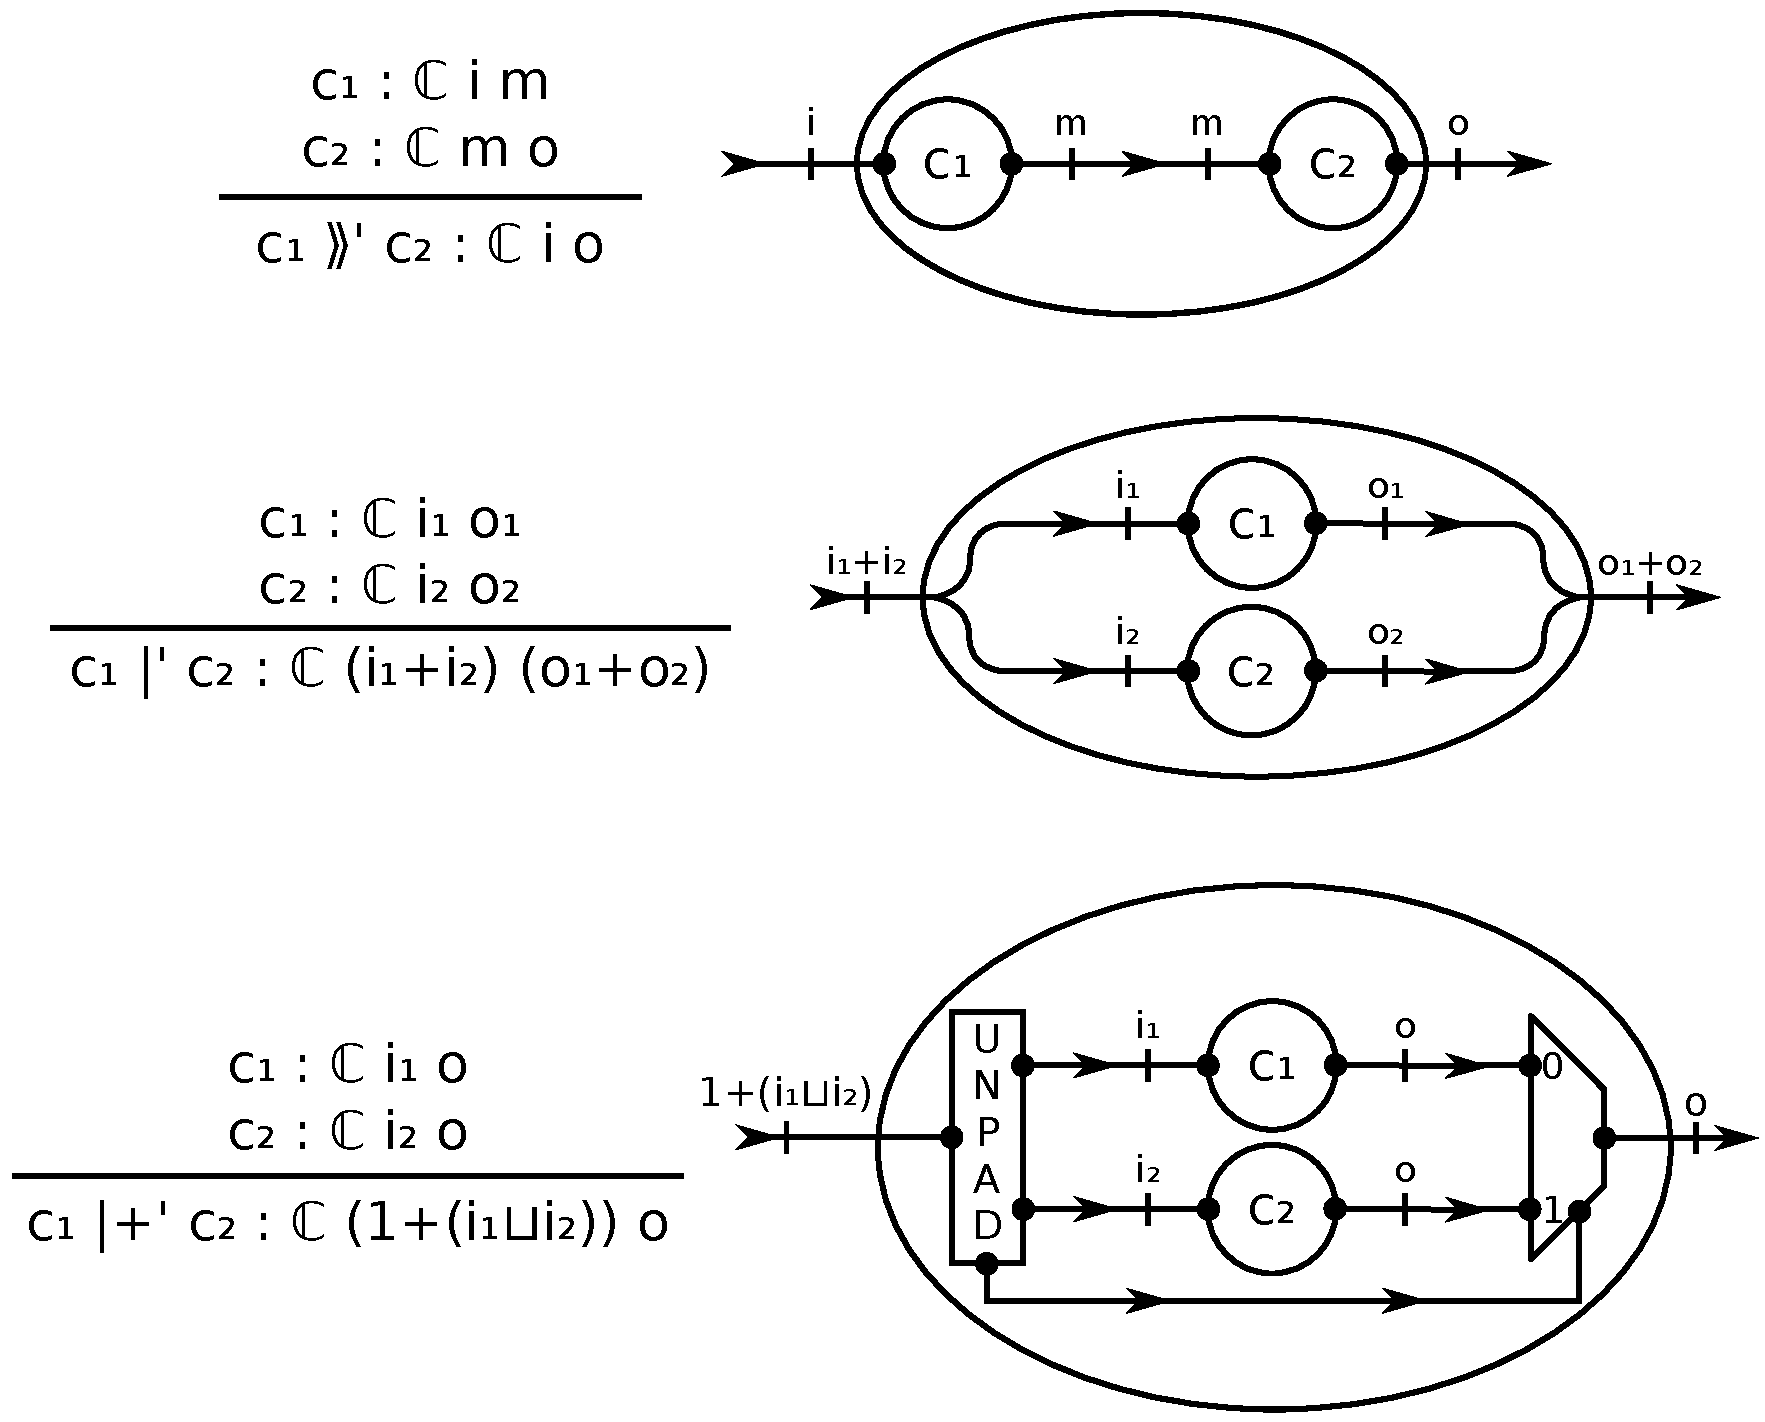
\includegraphics[width=0.93\textwidth]{imgs/semantics-syn-structural.pdf}}
                \caption{Synthesis semantics of structural circuit constructors.\label{fig:semantics-syn-structural}}
            \end{figure}

            In the sum case (\AI{\_|+'\_}), the \texttt{UNPAD} block only "slices" the input into three outputs:
            the tag (first bit) is used as the selector for the \emph{multiplexer}, and the other two outputs
            have, respectively, the first \AB{i₁} and \AB{i₂} bits of the input.
            The diagram on Figure~\ref{fig:semantics-syn-unpad} shows which slices of input go to each
            output of the \texttt{UNPAD} block in the sum case.

            \begin{figure}[h]
                \centering{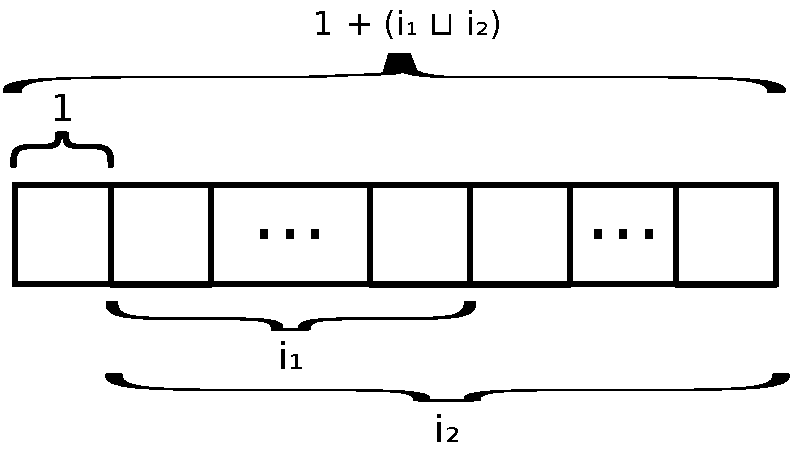
\includegraphics[width=0.60\textwidth]{imgs/semantics-syn-unpad.pdf}}
                \caption{How \texttt{UNPAD} "slices" its input into three outputs.\label{fig:semantics-syn-unpad}}
            \end{figure}

            Finally, it is important to emphasize that the labels \texttt{'0'} and \texttt{'1'}
            were used in the multiplexer only as a mnemonic device.
            The same remark applies to describing the information on the wires as "bits".
            In reality, any \AD{Atomic} type can flow through the wires, and any two \AD{Atom}s
            can label the inputs of the multiplexer (passed to \AI{\_|+'\_}).


        \subsection{Combinational simulation}
        \label{subsec:combinational-eval}
            %% Two types of evaluation: combinational and sequential
            %% Combinational eval requires a proof that the circuit contains no loops
            %%     Eval of a fundamental gate is just its \emph{definitional behaviour}

            As already mentioned in Section~\ref{sec:circuit-syntax},
            the \AF{comb'} predicate determines whether its circuit argument is \emph{purely combinational}.
            In fact, \AF{comb'} can be seen as one (very simple) semantics of circuits (\AD{ℂ'}).
            To recapitulate, here is the type of \AF{comb'}:

            \begin{center}
                \ExecuteMetaData[agda/latex/PiWare/Circuit/Core.tex]{comb-core-decl}
            \end{center}

            This predicate is used in several places in the Π-Ware library, particularly in what concerns
            the \emph{simulation} semantics.
            Purely combinational circuits have no notion of time or state, so their simulation semantics
            is modelled as just a function over \emph{words} (\AD{Atom} vectors).

            The Agda function giving a time-independent (combinational) semantics for circuits requires then
            that \emph{an element of type \AF{comb'}} be passed as (implicit) argument.
            Furthermore, this semantics of course depends on the \emph{gate library} and the
            \AD{Atom} type being used, which are parameters to the \AM{PiWare.Simulation.Core} module as a whole.
            Listing~\ref{lst:eval-core} shows the Agda code for the combinational simulation semantics:

            \begin{listing}[h]
                \centering{\ExecuteMetaData[agda/latex/PiWare/Simulation/Core.tex]{eval-core}}
                \caption{Agda code for the combinational simulation semantics of \AD{ℂ'}.\label{lst:eval-core}}
            \end{listing}

            First of all, notice the prime symbol on the function's name (\AF{⟦\_⟧'}),
            indicating that it concerns \emph{low-level} circuits (\AD{ℂ'}).
            From the cases for fundamental constructors, we highlight the usage of the \AF{spec}
            function from the chosen gate library, returning the specification function for a given gate.
            Furthermore, the \AI{DelayLoop} case can be \emph{discharged}, i.e.,
            it is not necessary to provide a definition in this case,
            as \AF{comb'} \AY{(}\AI{DelayLoop} \AB{c}\AY{)} evaluates to \AD{⊥}
            and – by definition – no elements of this type can be constructed.

            The cases for structural constructors are somewhat straightforward.
            Sequencing (\AI{\_⟫'\_}) is interpreted just as function composition.
            In the parallel composition (\AI{\_|'\_}) case, first the input vector is \emph{splitted}, creating a pair.
            Then the \AF{map} function over pairs is used, to apply (respectively) the semantics of \AB{c₁}
            and \AB{c₂} over each element of the pair.
            Finally, both transformed pair elements are concatenated to build the output.
            In the sum (\AI{\_|+'\_}) case, the \AF{untag} function uses the first atom of the input
            to decode it into a sum.
            Then the sum destructor (\AF{[\_,\_]'}) is used with the appropriate functions
            (semantics of \AB{c₁} and \AB{c₂}) to build the output accordingly.

            Notice how the (implicit) arguments of type \AF{comb'} \AB{c} are matched against and passed.
            In the cases for structural constructors, we know that – by definition – the
            \emph{whole circuit is combinational if and only if all its subcircuits are combinational}.
            Therefore, we can pattern match with the \emph{pair constructor} (\AB{p₁} \AI{,} \AB{p₂}),
            and pass each of \AB{p₁} and \AB{p₂} to the calls of \AF{⟦\_⟧'} on the subcircuits.

            \subsubsection{High-level combinational simulation}
            Analogous to the dichotomy between low-level \emph{circuits} (\AD{ℂ'}) and high-level ones (\AD{ℂ}),
            there are also both low and high-level simulation
            semantics~\footnote{There is no such "high-level" concept for the \emph{synthesis} semantics,
                as it concerns actual hardware.}.

            While the low-level simulation semantics (\AF{⟦\_⟧'}) maps a low-level circuit (\AD{ℂ'})
            to a function over \emph{words},
            the high-level simulation semantics (\AF{⟦\_⟧} – shown in Listing~\ref{lst:eval})
            maps a high-level circuit (\AD{ℂ}) to a function over arbitrary (synthesizable) Agda types.

            \begin{listing}[h]
                \centering{\ExecuteMetaData[agda/latex/PiWare/Simulation.tex]{eval}}
                \caption{Simulation semantics for high-level circuits (\AD{ℂ}).\label{lst:eval}}
            \end{listing}


        \subsection{Sequential simulation}
        \label{subsec:sequential-eval}
            %% For sequential circuits we use a \emph{causal stream semantics}
            %%     Current output depends on the current input and (possibly) on the past inputs
            %%     \emph{Different} than plain Stream functions
            %% There's also an eval function which allows the circuit to be viewed as function from Stream to Stream

            So-called \emph{sequential} circuits have an internal state,
            and their behaviour is \emph{history-dependent}:
            The current value of a circuit's output depends not only on the current input,
            but also on the history of previous inputs.
            Therefore, to simulate these circuits, there is the need of some concept of \emph{time dimension}
            where the values of inputs and outputs are situated.

            Π-Ware supports modelling and simulating a specific class of sequential circuits,
            namely \emph{synchronous} sequential circuits.
            In synchronous sequential circuits, state transitions in all memory elements happen
            at the same time, and they can only happen at the (rising or falling) \emph{edge}
            of a global clock circuit.
            Because of this \emph{discrete} nature of signals in synchronous circuits,
            they are usually modelled as \emph{streams} in hardware \acp{DSL}.
            This is also the way in which sequential simulation works in Π-Ware:
            it converts a circuit into a function over streams.

            Listing~\ref{lst:eval-seq-core-decl} shows the type of the semantic function for
            sequential simulation of low-level (\AD{ℂ'}) circuits:

            \begin{listing}[h]
                \centering{\ExecuteMetaData[agda/latex/PiWare/Simulation/Core.tex]{eval-seq-core-decl}}
                \caption{Type signature of the semantic function for low-level sequential simulation.
                    \label{lst:eval-seq-core-decl}}
            \end{listing}

            This type signature differs from the purely combinational case (depicted in Listing~\ref{lst:eval-core})
            in only two important ways:

            \begin{itemize}
                \item There is no argument of type \AF{comb'} \AB{c} anymore
                    requiring the circuit to be purely combinational.
                \item The result of evaluating the circuit is now "lifted" to the \AD{Stream} setting,
                    that is, it becomes
                    \AD{Stream} \AY{(}\AD{W} \AB{i}\AY{)} \AY{→} \AD{Stream} \AY{(}\AD{W} \AB{o}\AY{)}.
                    instead of \AD{W} \AB{i} \AY{→} \AD{W} \AB{o}.
            \end{itemize}

            The implementation of the history-dependent behaviour needed in sequential simulation
            uses so-called \emph{causal streams}~\cite{essence-dataflow-programming}.
            Even though the type
            \AD{Stream} \AY{(}\AD{W} \AB{i}\AY{)} \AY{→} \AD{Stream} \AY{(}\AD{W} \AB{o}\AY{)}
            is convenient as an \emph{interface} to interact with sequential circuits, it does not
            reflect accurately the way in which synchronous sequential circuits actually work.

            The type of a general stream function (\AD{Stream} \AB{α} \AY{→} \AD{Stream} \AB{β})
            can be read as:

            \begin{quote}
                Given an infinite sequence of values of type \AB{α},
                produce an infinite sequence of values of type \AB{β}.
            \end{quote}

            As such, a general stream function has no notion of \emph{current} value, neither of past,
            and it \emph{can} "look ahead", that is, use future input values to calculate the next output value.
            One example of such a future-dependent behaviour.
            %% TODO: example of future-dependent stream function

            \subsubsection{Causal Streams}
            \label{subsubsec:causal-streams}
            Therefore, in Π-Ware, the semantic function for sequential circuits is built upon an
            auxiliary definition, which gives \emph{one step} of a causal stream function, i.e,
            given the current and past values, it produces \emph{the next} value on the output.
            First, let's start by introducing (in Listing~\ref{lst:causal-types}) the types used to model causal streams.

            \begin{listing}[h]
                \centering{\ExecuteMetaData[agda/latex/Data/CausalStream.tex]{causal-context}}
                \newline
                \centering{\ExecuteMetaData[agda/latex/Data/CausalStream.tex]{causal-step}}
                \caption{Types used to model causal streams.\label{lst:causal-types}}
            \end{listing}

            We represent a \emph{causal context} with values of type \AB{α} by \AD{Γc} \AB{α}.
            It contains the current \emph{and} past values of the stream.
            We use Agda's \emph{non-empty lists} to implement the context, which means
            the current value is always present, even though there might be no past.


    \section{Proving circuit properties}
    \label{sec:proving-circuit-properties}
